
\begin{frame}
		\frametitle{Distributed Sort}
		\begin{figure}
				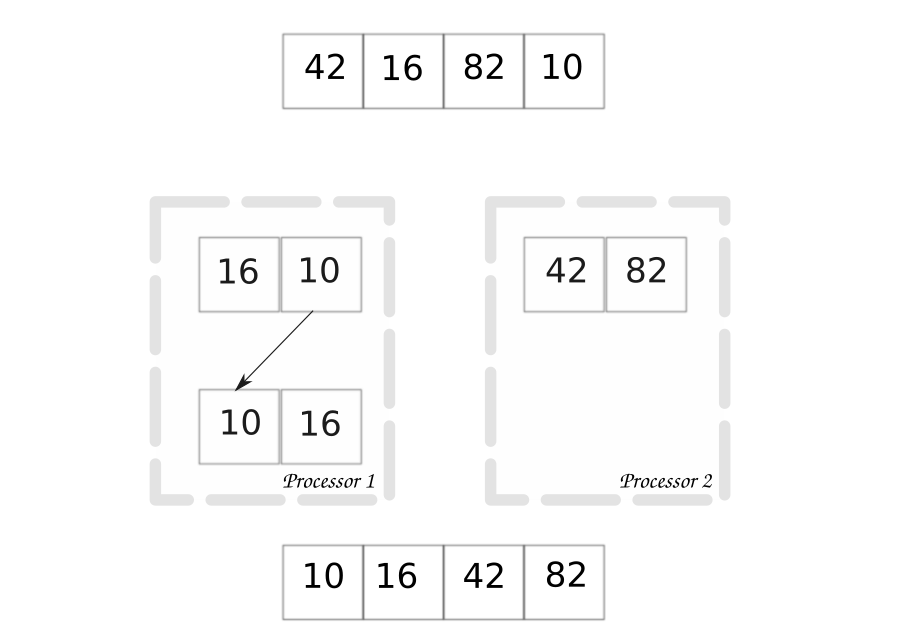
\includegraphics[width=0.8\linewidth]{figures/diagrams/sort/parallelsort}
		\end{figure}
\end{frame}

\begin{frame}
		\frametitle{Distributed Sort}
		\begin{figure}
			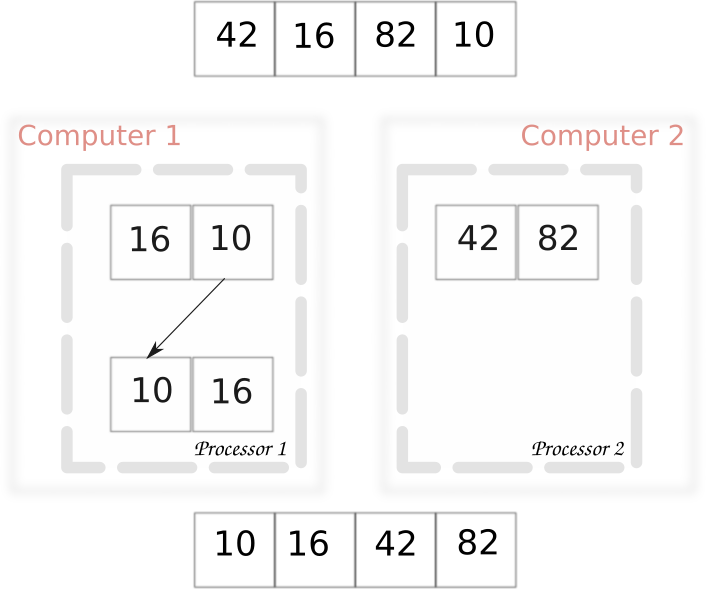
\includegraphics[width=0.7\linewidth]{figures/diagrams/sort/distributedsort}
		\end{figure}
\end{frame}

\begin{frame}
		\frametitle{Distributed CLI}
		mpirun - CLI mpi examples
\end{frame}

\begin{frame}[fragile]
		\frametitle{Distributed Code}
		\begin{verbatim}
		library(pbdMPI)

		init()
		.comm.size <- comm.size()
		.comm.rank <- comm.rank()

		x <- 5

		if (.comm.rank == 0) {
		    send(x)
		} else {
		    y <- recv(x)
		}

		comm.print(y,rank.print=1)
		finalize()
		\end{verbatim}
\end{frame}

\begin{frame}[fragile]
		\frametitle{Distributed Code}
		\begin{verbatim}
		init()
		.comm.size <- comm.size()
		.comm.rank <- comm.rank()

		x <- sample(1:1000, 50, replace = T)

		x_global <- 0
		y <- sum(x)

		x_global <- reduce(y, op="sum")

		comm.print(x_global, rank.print==0)
		finalize()
		\end{verbatim}
\end{frame}

\begin{frame}
		\frametitle{Observed Speedup}
		observed speedup ( figure )
\end{frame}

\begin{frame}
		\frametitle{Efficient Memory Use}
		\begin{figure}
				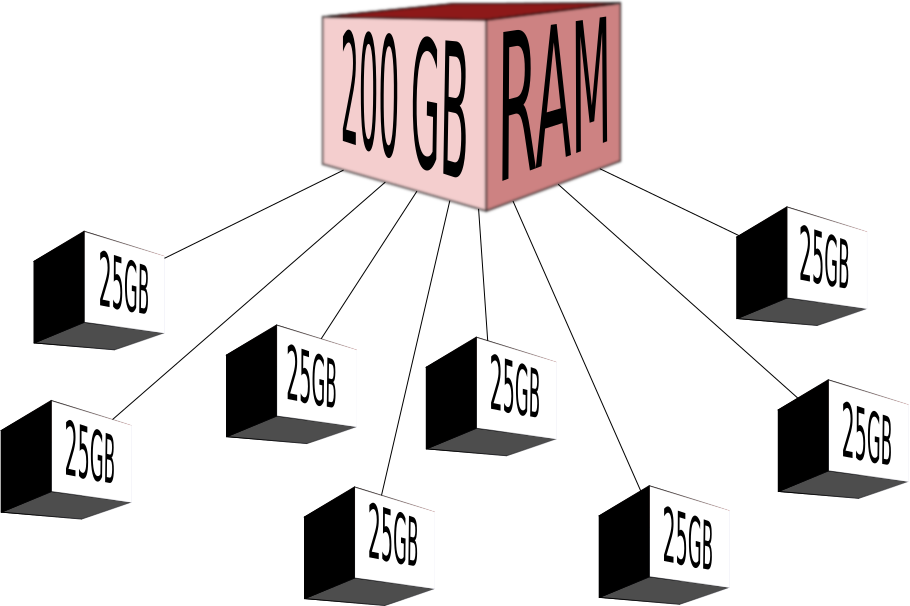
\includegraphics[width=0.8\linewidth]{figures/diagrams/splitmem/memsplit}
		\end{figure}
\end{frame}

\begin{frame}
		\frametitle{MPI is faster}
		\begin{figure}
				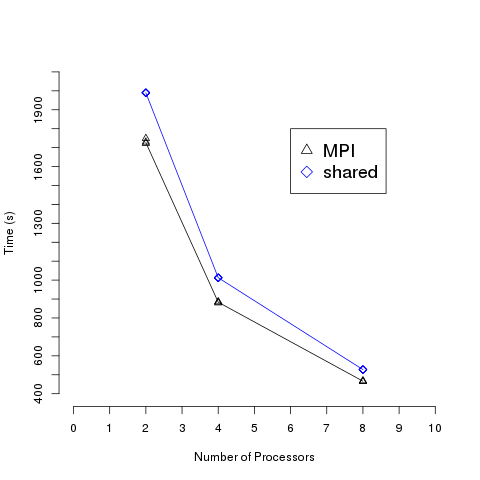
\includegraphics[width=0.65\linewidth]{figures/diagrams/comparison/comparison}
		\end{figure}
\end{frame}

\begin{frame}
		\frametitle{MPI infrastructure requirements}
		\begin{figure}
				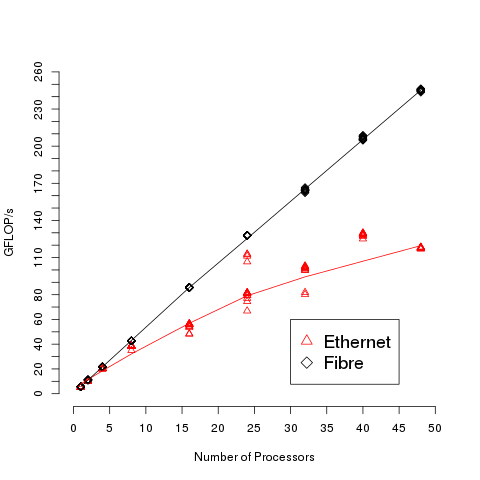
\includegraphics[width=0.65\linewidth]{figures/diagrams/connection/connection}
		\end{figure}
\end{frame}


